\documentclass[11pt]{article}
    \title{\textbf{Práctica 4}}
    \author{Adrián Racero Serrano}
    \date{}
    
    \addtolength{\topmargin}{-2cm}
    \addtolength{\textheight}{3cm}
\usepackage{graphicx}
\usepackage{whilecode2}
\usepackage{algorithmic}
\usepackage{verbatim}
\begin{document}

\maketitle
\thispagestyle{empty}

\section*{Ejercicio 1}
\begin{whilecode}[H]
$minDiverge=(0, s)$
\\
$s:$
\\
 $X_1 \Assig X_1 + 1$\;
 \While{$X_1 \not = 0$}{

  $X_1 \Assig X_1$\;

 }

\end{whilecode}

\begin{figure}[htp]
\centering
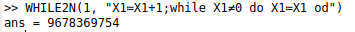
\includegraphics[scale=0.70]{while2n.png}
\end{figure}

\newpage
\section*{Ejercicio 2}

\verbatiminput{allVector.m}

\begin{figure}[htp]
\centering
\includegraphics[scale=0.55]{Ejecución_allVector.png}
\end{figure}

\newpage
\section*{Ejercicio 3}

\verbatiminput{allProgramWhile.m}
\begin{figure}[htp]
\centering
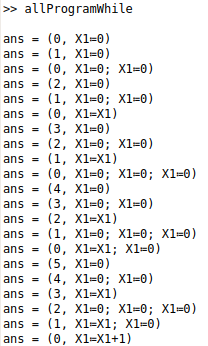
\includegraphics[scale=0.60]{allProgramExecution.png}
\end{figure}
\end{document}

